% !TeX root = ../UrrutiaAnguiano_CandidaturaDefensa.tex
% !TeX spellcheck = es_MX 

\section{Avances en caracterización no intrusiva}
	\subsection{Efectos debido al sustrato}


\begin{frame}{Avances en caracterización no intrusiva}
	{\textoverline{¿Esparcimiento múltiple o interacción con partícula imagen?}}
	\begin{columns}
		\column{.3\textwidth}
		\centering	
			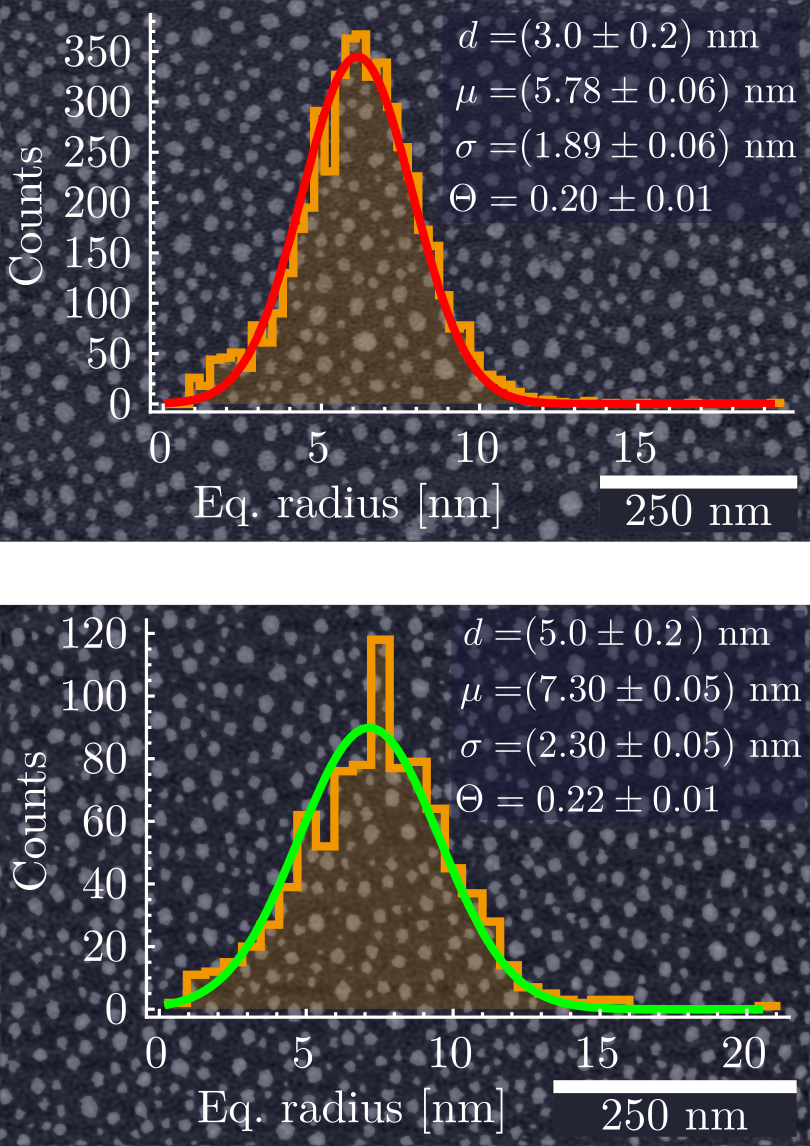
\includegraphics[scale = 1]{img/4-NonInt/g6.png}
		\column{.4\textwidth}
		\centering
			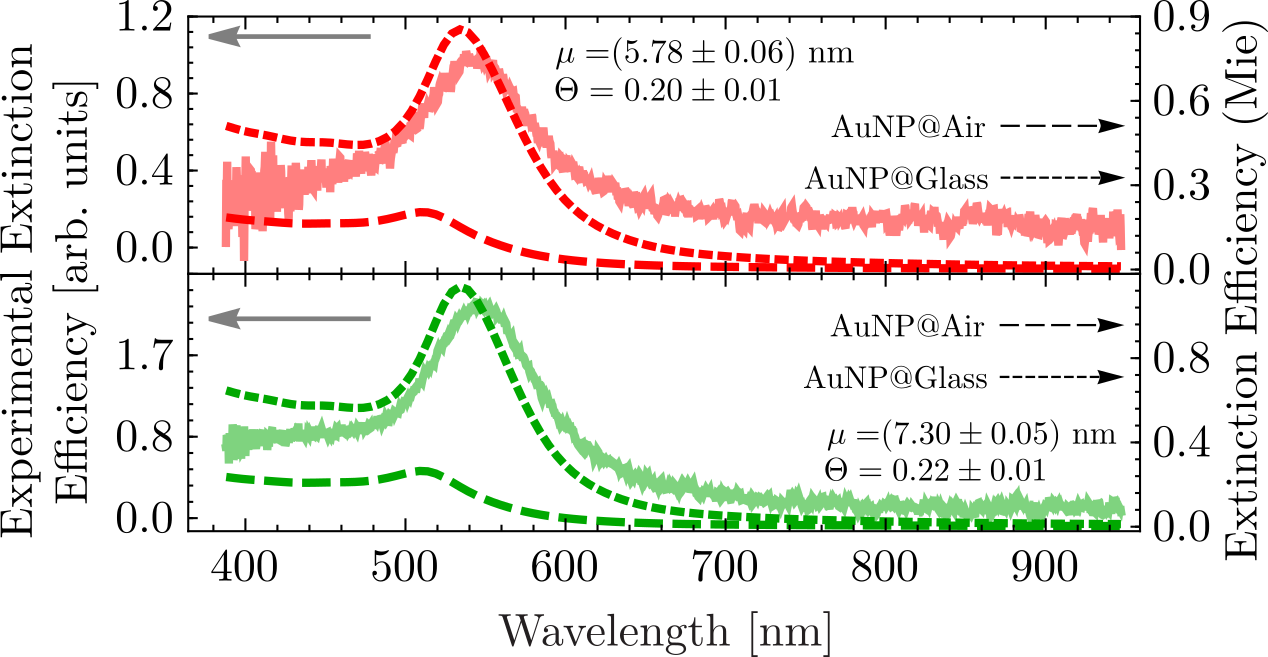
\includegraphics[scale = 1]{img/4-NonInt/g3.png}
		\column{.3\textwidth}
			\centering
			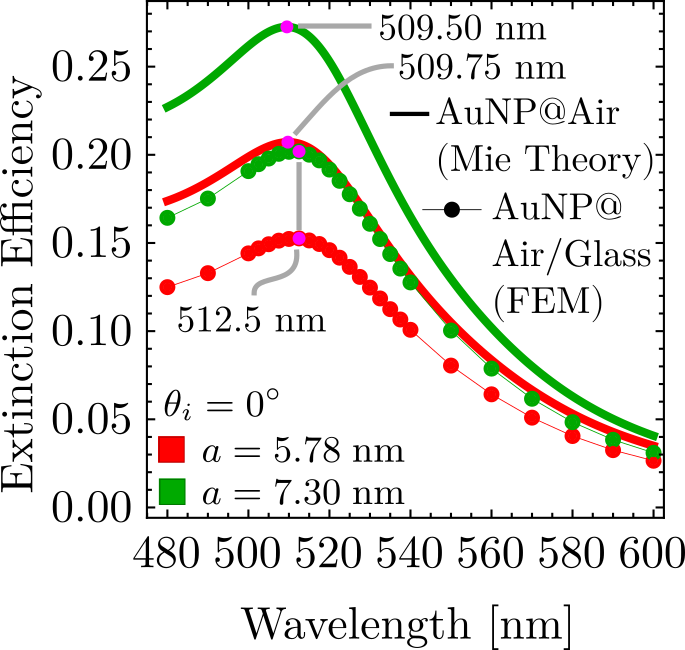
\includegraphics[scale = 1]{img/4-NonInt/g4.png}
	\end{columns}
\end{frame}

\begin{frame}{Avances en caracterización no intrusiva}
	{\textoverline{Minimización del error por descenso de gradiente}}
		\centering	
		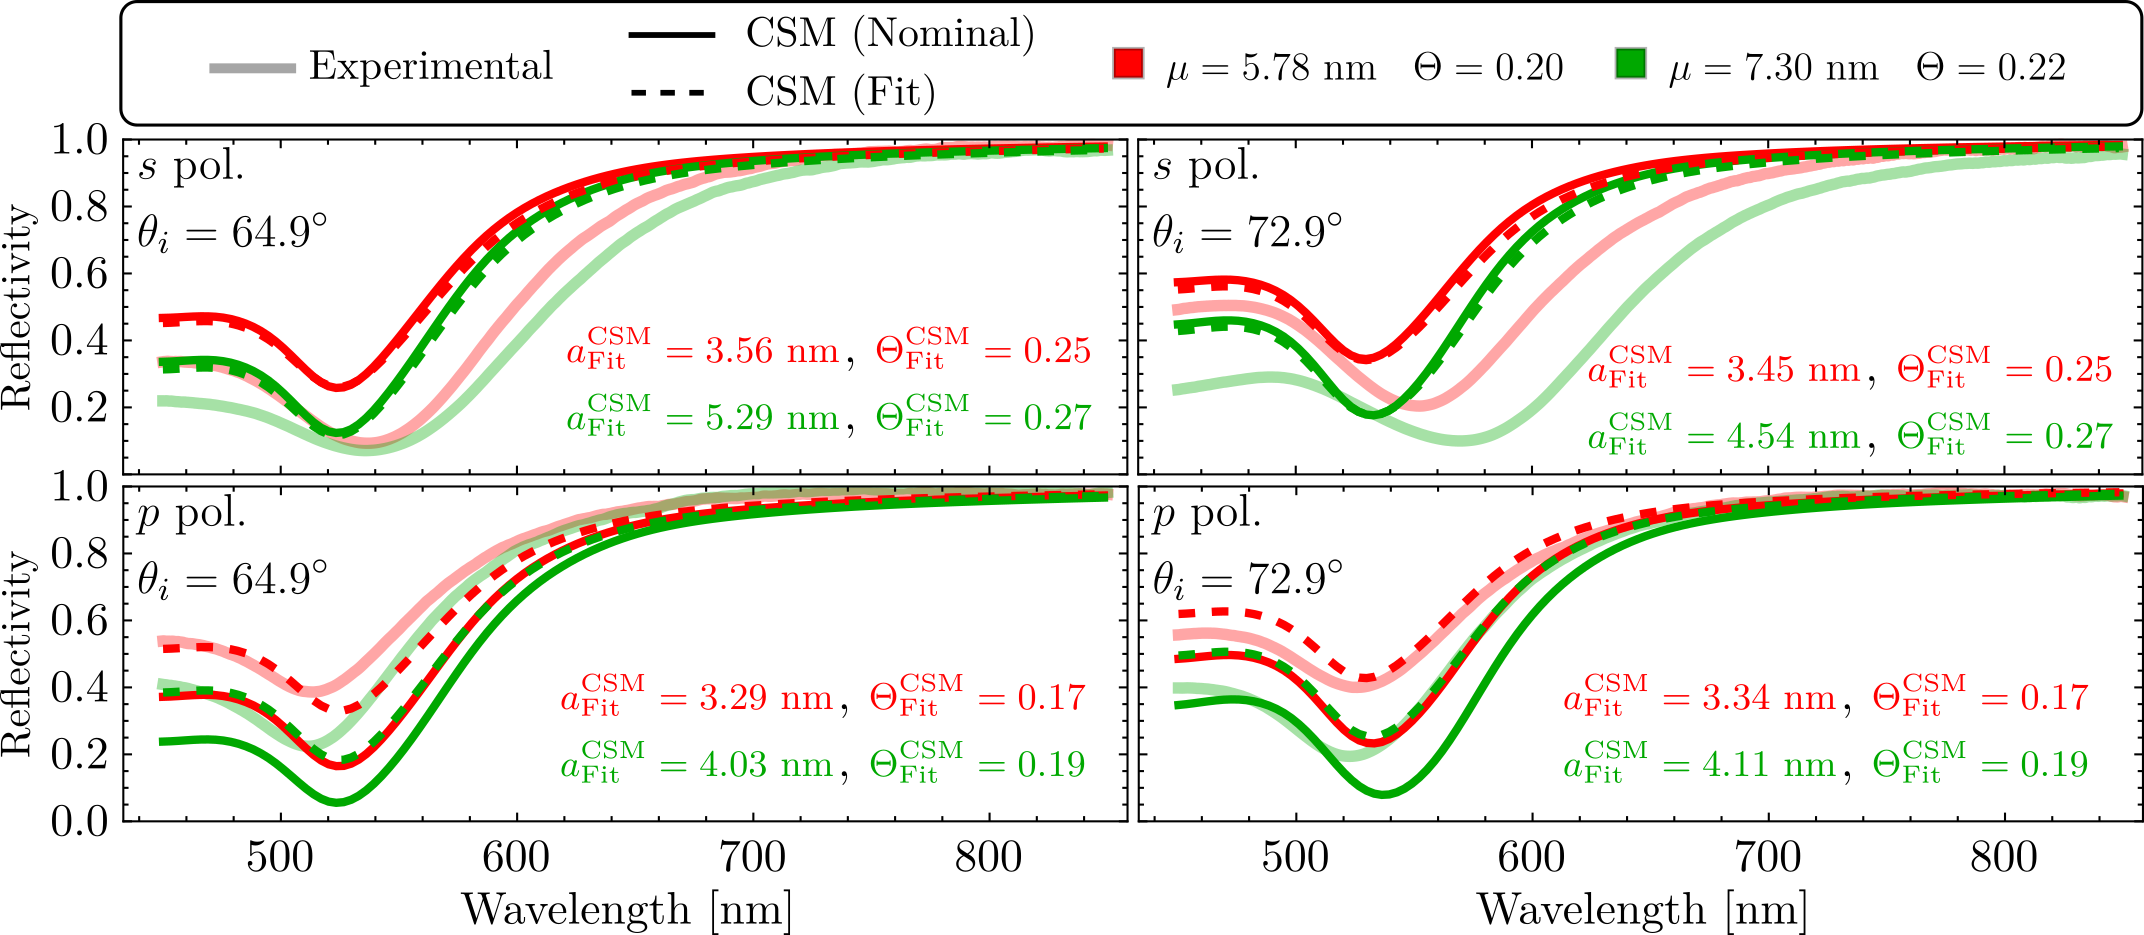
\includegraphics[scale = 1.1]{img/4-NonInt/Fig-Fit.png}
\end{frame}

\begin{frame}{\underline{Avances en caracterización no intrusiva}}
	{Determinación del incrustamiento parcial}
\centering
	\begin{columns}
	\column{\squeezetwo}
	\centering	
	$$V_\text{above}^\text{semi-sphere} = \frac43 \pi a^3 \left[\frac12 - \frac34\left(\frac{h}{a}\right) + \frac14\left(\frac{h}{a}\right)^3\right] = \frac43 \pi (a_\text{Fit}^\text{CSM})^3 = V_\text{eq}$$
	$$	\eta\left(\frac{h}{a}\right) = \frac12 - \frac34\left(\frac{h}{a}\right) + 
	\frac14\left(\frac{h}{a}\right)^3 -  \left(\frac{a_\text{Fit}^\text{CSM}}{a}\right)^3
	=0$$
	\vskip5mm
	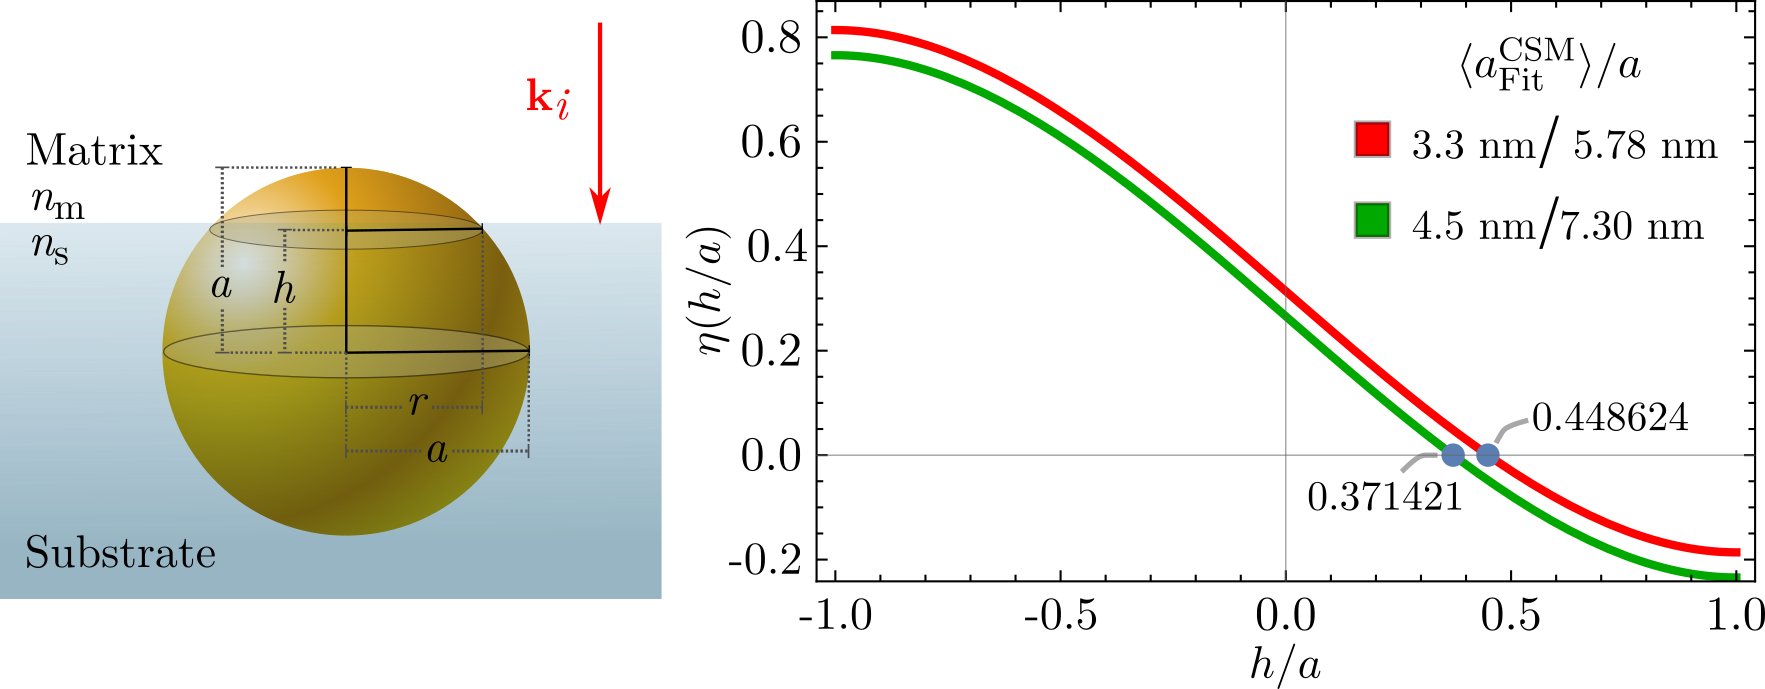
\includegraphics[scale = 1]{img/4-NonInt/Fig-Embedding.png}
	\column{\squeezethree}
	\centering\vskip-10mm
	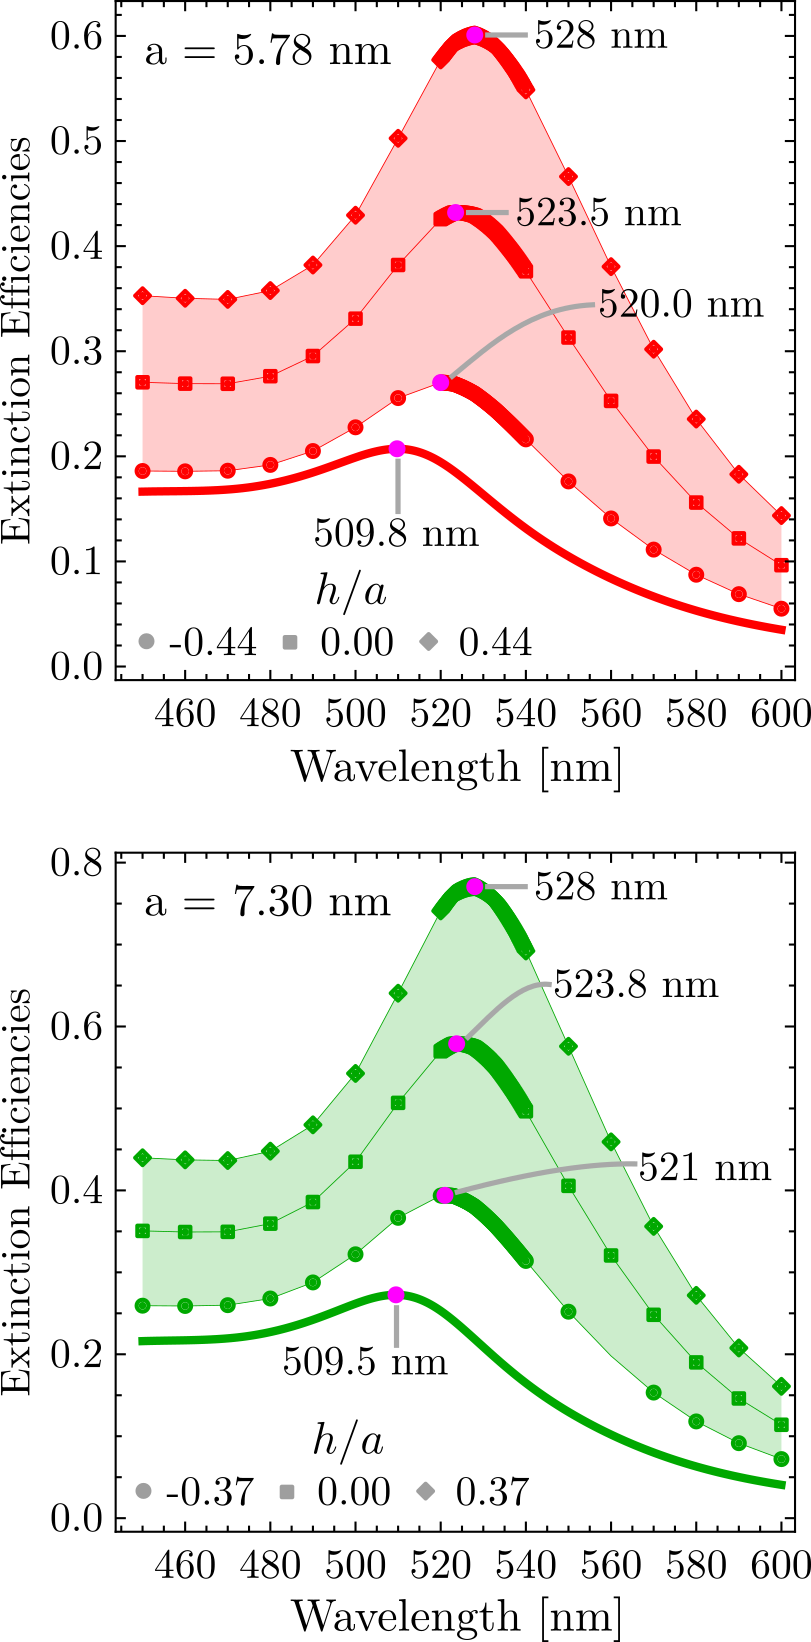
\includegraphics[scale = 1]{img/4-NonInt/Fig-CextMieEmb.png}
\end{columns}
\end{frame}

\begin{frame}{\underline{Avances en caracterización no intrusiva}}
	{Interacción entre pares de partículas}
	\centering
	\begin{columns}
		\column{\squeezetwo}
		\centering	
		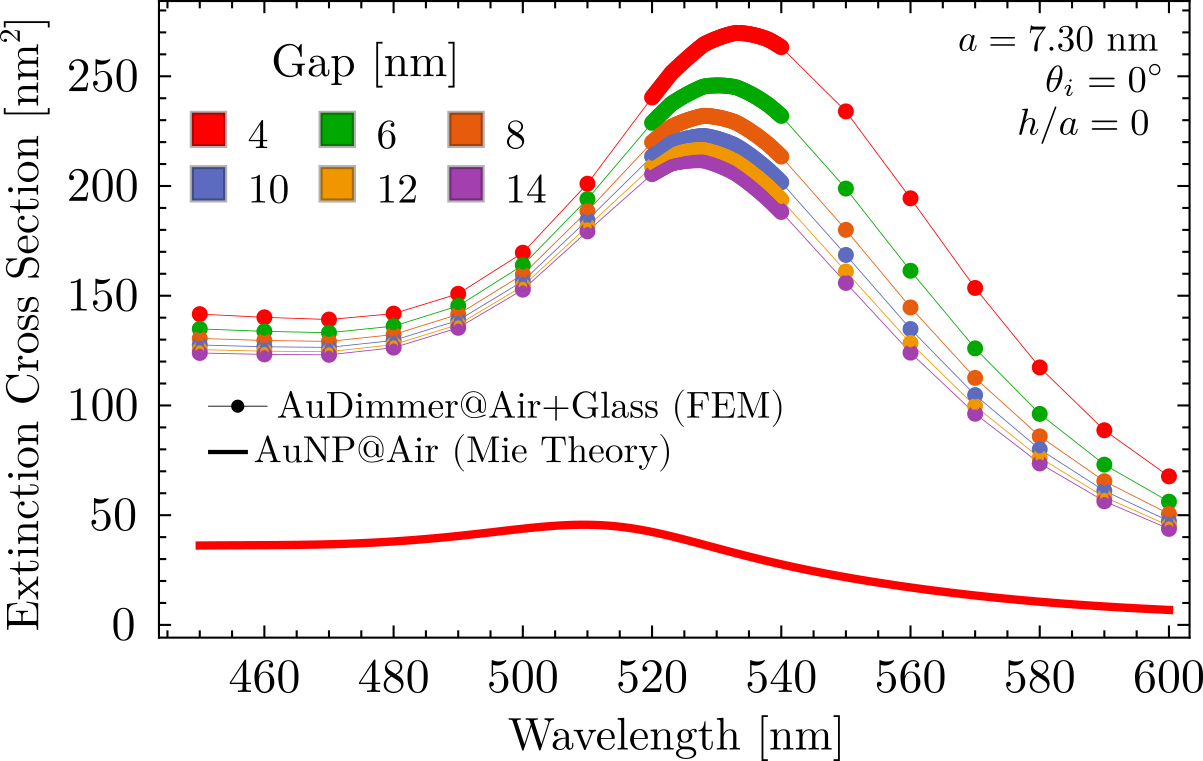
\includegraphics[scale = 1]{img/4-NonInt/g1425.png}
		\column{\squeezetwo}
		\centering\vskip-10mm
		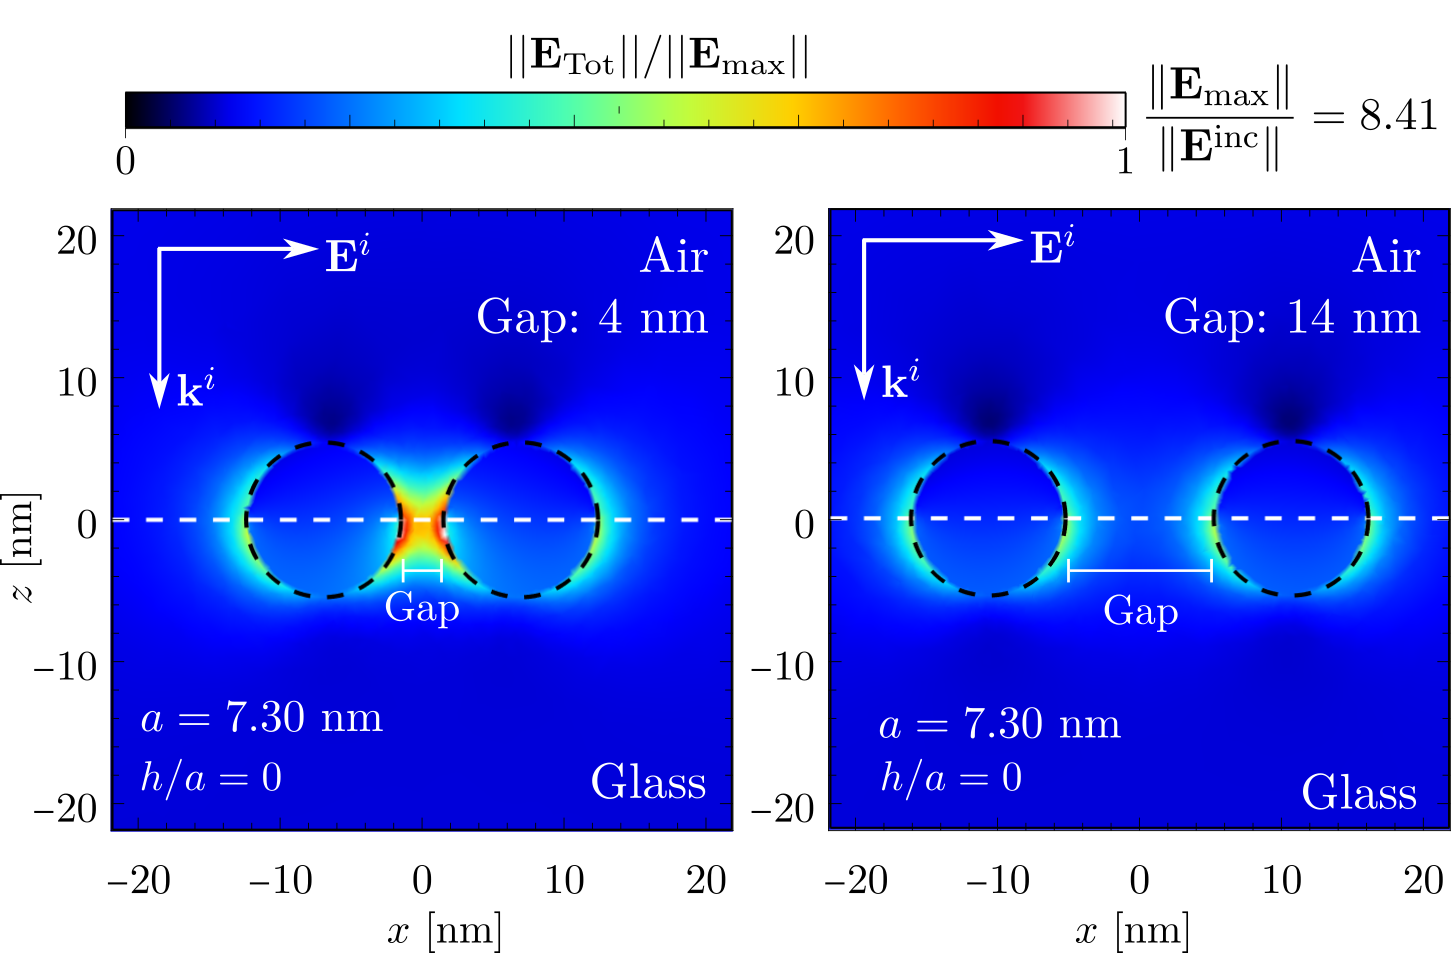
\includegraphics[scale = 1]{img/4-NonInt/g1424.png}
	\end{columns}
\end{frame}

\begin{frame}{Avances en caracterización no intrusiva}
	{\textoverline{Primeras mediciones de incrustamiento parcial}}
	\centering
	\begin{columns}
		\column{\squeezethree}
		\centering	
		
\includegraphics[scale = 1]{img/4-NonInt/Fig-Extinction.png}
		\column{\squeezetwo}
		\centering
		
\includegraphics[scale = 1]{img/4-NonInt/Fig-ATRThick.png}
	\end{columns}
\end{frame}

